\documentclass{article}
\usepackage[margin=1in]{geometry}
\usepackage{amsmath, amssymb, amsthm}
\usepackage{enumitem}

% Inputting Python code
\usepackage[dvipsnames]{xcolor}
\definecolor{textblue}{rgb}{.2,.2,.7}
\definecolor{textred}{rgb}{0.54,0,0}
\definecolor{textgreen}{rgb}{0,0.43,0}
\usepackage{upquote}
\usepackage{listings}
\lstset{
    language=Python, 
    tabsize=4,
    basicstyle={\small\ttfamily},
    keywordstyle=\color{textblue},
    commentstyle=\color{textgreen},
    stringstyle=\color{textred},
    frame=none,
    columns=fullflexible,
    keepspaces=true,
    showstringspaces=false,
    xleftmargin=-1cm, % manual adjustment, figure out permanent solution
}

%Images
\usepackage{graphicx}
    \usepackage{float}
    \usepackage[labelsep=period]{caption}

%Formatting and Spacing
\setitemize[1]{noitemsep, parsep = 5pt, topsep = 5pt}
\setenumerate[1]{label = (\alph*), parsep = 1pt, topsep = 5pt}
\setlength\parindent{0pt}
\linespread{1.15}

%Formatting and Spacing
\usepackage{enumitem}
\setitemize[1]{noitemsep, parsep = 5pt, topsep = 5pt}
\setenumerate[1]{label = (\alph*), parsep = 1pt, topsep = 5pt}
\setlength\parindent{0pt}
\linespread{1.1}

% title
\title{\vspace{-1cm}CS 2051: Honors Discrete Mathematics \\Spring 2023 Homework 3 Supplement}
\author{Sarthak Mohanty}
\date{}

\begin{document}

\maketitle

\section{Overview}

    In this supplement, you'll learn to automate rules of inference through code. You'll also learn about the infamous \textbf{boolean satisfiability problem}, and see one of its many applications through the equally famous \textbf{four color theorem}.

\section*{Part 1: Rules of Inference}
    As you've seen on this homework, rules of inference are difficult to get right. With lots of variables, it takes a lot of work and time to check if a conclusion is valid. However, with a little bit of programming, we can speed this up a bit. 
    
    \textbf{In this part, you'll implement the following function:}
    
    \begin{itemize}
        \item \lstinline{infer(inference_rules, conclusion)} This method takes in inference rules in the form 
    \end{itemize}

    Since you're actually quite familiar with manipulating propositions of this form from the last supplement, this 


\section*{Part 2: The Boolean Satisfiability Problem (SAT)}

The best way to understand the SAT problem is with an example. Consider the following formula:



Assume you are in charge of elections in a society. Elections in this society work as follows: there are $n$ candidates, and any number of them, from 0 (nobody) to $n$ (everybody) can be elected as the result of the elections. Each voter provides a list of candidates they want elected and candidates they want not elected. For example, if we call the candidates A, B and C, then one vote might be "A, B, not C". We say a voter will be satisfied with the results of the election if at least one of his/her preferences is met. For example, the voter with the "A, B, not C" vote will be satisfied if either A or B is elected, or if C is not elected. To be clear, that voter will be happy even if nobody is elected because one of the preferences is "not C" which is met if we do not pick anyone. It's also possible to receive an empty vote which means that the voter will not be satisfied regardless of who is elected.


We can represent this problem in logical form:


\textbf{In this part, you'll implement the following function:}
    
    \begin{itemize}
        \item 
    \end{itemize}

\section*{Part 3: Four Coloring Problem}


    This lends itself to a simple decision problem: given a map, is it possible to color it using 4 or less colors such that no two neighboring regions are the same color? The four color theorem is then true if and only if the answer to this decision problem is always true (provided the input map meets the requirements of a planar graph, a detail we are not too concerned with here). As input, we will take the number of regions $n$, and assume the regions are labeled using numbers 1 to $n$, and a list of neighboring regions of the form ${i,j}$ with $i\neq j$, indicating regions $i$ and $j$ are neighbors. Let us use colors red (R), blue (B), green (G), and yellow (Y) to color the regions. Our variables are going to be $R_i$, $B_i$, $G_i$ and $Y_i$, for $1 \leq i \leq n$, indicating that region $i$ is colored red, blue, green, or yellow, respectively.


    \vspace{1.5mm}
    Next, we need to construct the right set of clauses such that if all of them are satisfied, then we have a proper coloring of the map. Specifically, we need every region to be colored, and we need no two neighboring regions to be the same color. First, let us construct the clauses that will make sure every region has one and only one color assigned to it. For this, we need to make sure only one of $R_i$, $B_i$, $G_i$ or $Y_i$ is picked for our assignment at a time. We can express this in terms of $K$ clauses for each region $i$. First, we add $R_i \lor B_i \lor G_i \lor Y_i$ as a clause, which ensures that region $i$ gets at least one color assigned to it. Then for pair of colors, say $R$ and $B$, we add the clause $\neg R_i \lor \neg B_i$, which basically says "not both of $R_i$ and $B_i$ can be picked at the same time", effectively making sure that exactly one color is assigned to each region. Finally, for any two neighboring regions, say $i$ and $j$, and each color, say $R$, we add the clause $\neg R_i \lor \neg R_j$ which says not both of $i$ and $j$ can be colored red.


    \textbf{In this part, you'll implement the following function:}
    \begin{itemize}
        \item \lstinline{fourColoringtoSAT(neighbors)}: This problem takes in \lstinline{neighbors} (a representation of the 4COLOR problem) and returns an equivalent proposition constructed using the method outlined above.
    \end{itemize}

    \begin{figure}[htbp]
        \centering
        \hspace{1cm}
        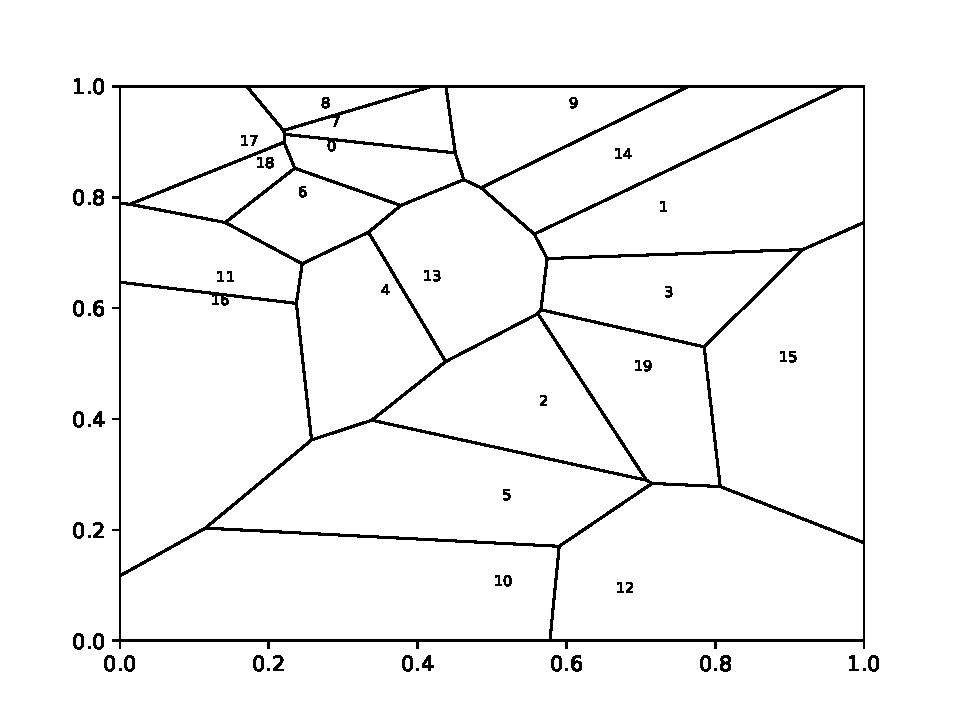
\includegraphics[scale = .6]{sp23/hw-supplements/hw3-supp-draft/blank_map.pdf}
        \caption{Blank Map.}
        \label{fig:blank_map}
    \end{figure}


    \begin{figure}[htbp]
        \centering
        \hspace{1cm}
        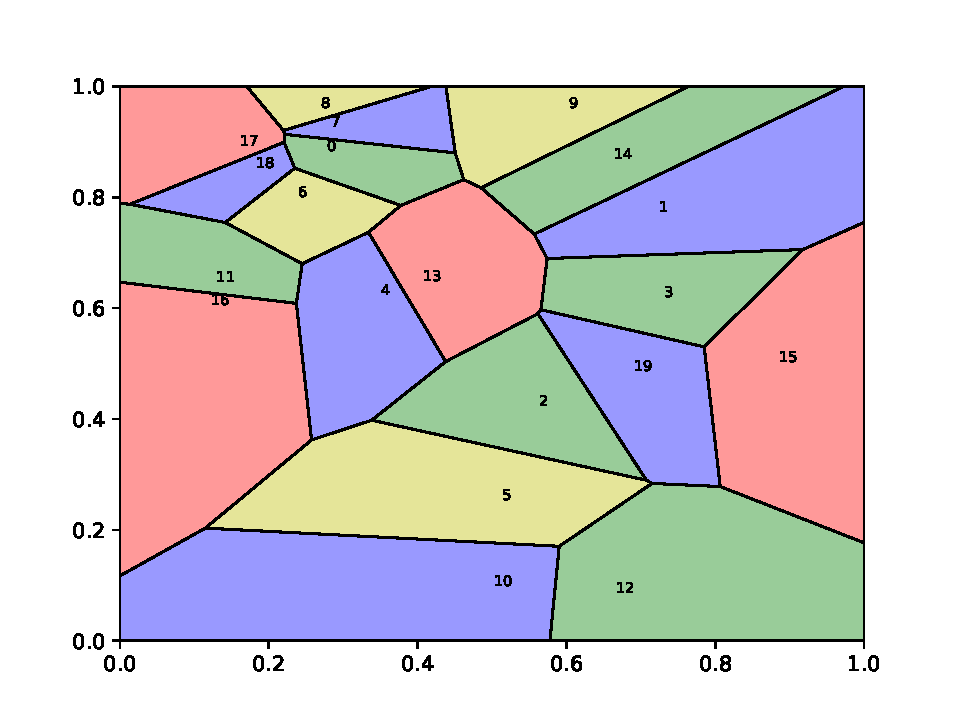
\includegraphics[scale = .6]{sp23/hw-supplements/hw3-supp-draft/colored_map.pdf}
        \caption{Colored map}
        \label{fig:colored_map}
    \end{figure}

\section{Submission Instructions}
    After you fill the appropriate methods, submit the following files to Gradescope and make sure you pass all test cases:
    \begin{itemize}
        \item \lstinline{inference.py}
        \item \lstinline{SAT.py}
        \item \lstinline{fourCOLOR.py}
    \end{itemize}

    \vspace{3mm}
    \textbf{Note: The autograder may not reflect your final grade on the assignment. We reserve the right to run additional tests during grading.}
    


\end{document}